\subsubsection*{System Architecture: Microservices and Modular Monolithic}
System architecture defines the macroscopic structure of a software system, organizing its major components, inter-process communication, and load distribution. Given the necessity of building an intelligent system responsible for transferring, managing, and indexing massive volumes of educational materials, a monolithic architecture—where the entire application is compiled and deployed as a single unified binary—quickly becomes a massive bottleneck. To mitigate this, the system adopts a {Microservices Architecture}.

Microservices is a design paradigm in which a complex application is decoupled into a suite of small, autonomous, and loosely coupled services. Each service is dedicated to a specific business domain, operates in its own isolated process, and interacts with other services via lightweight protocols (typically REST APIs or message brokers like RabbitMQ/Kafka). 

\begin{figure}[H]
    \centering
    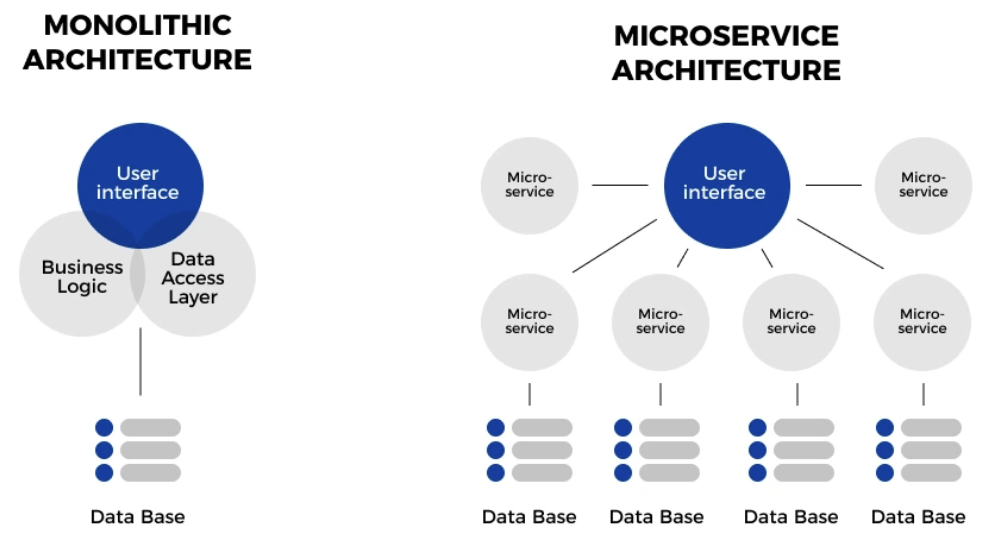
\includegraphics[width=0.7\textwidth]{Images/fundamental/micro.png}
    \vspace{12pt}\caption{Comparison of Microservice and Monolithic architecture}\label{fig:micro_vs_mono}
\end{figure}

The adoption of Microservices is fundamentally driven by the need to isolate distinct computational workloads. In an AI-driven educational platform, integrating compute-intensive tasks (like LLM inference and embedding generation) with I/O-intensive tasks (like API routing and user authentication) within the same process leads to resource starvation. Decomposing these into microservices yields critical structural advantages:

\begin{itemize}
    \item {Independent and Asymmetrical Scalability:} This is the most crucial advantage for AI systems. Microservices allow the architecture to scale heterogeneously. Heavy, GPU-bound inference services can be scaled vertically (allocating more VRAM) or horizontally (adding more instances) independently of the lightweight frontend and routing services. This ensures that a spike in users uploading documents does not unnecessarily drain the resources allocated to real-time chat inference, optimizing overall hardware utilization.
    
    \item {Fault Isolation and Blast Radius Containment:} In a distributed microservices ecosystem, failures are strictly contained within their respective domains. If the computationally heavy LLM generation service crashes due to an Out-Of-Memory (OOM) error, the blast radius is limited. The API Gateway, user authentication services, and database layers remain fully operational, ensuring high system availability and allowing users to continue browsing content while the AI service automatically restarts.
    
    \item {Technological Flexibility (Polyglot Programming):} Microservices eliminate the constraint of being locked into a single technology stack, allowing engineers to select the optimal tool for each specific task. For instance, AI agents and data processing pipelines are implemented in Python to leverage its rich machine learning ecosystem (PyTorch, LangChain). Simultaneously, the API gateway or real-time notification services might utilize high-concurrency, compiled languages like Go or Node.js. This polyglot approach ensures maximum performance efficiency across the entire application lifecycle.
\end{itemize}

\subsection{Technology Stack and Frameworks}


\subsubsection*{Frontend Development}
Frontend development is critical as it represents the intersection between the system's logic and human interaction. It focuses primarily on user experience, translating raw data into an accessible, responsive interface. The goal is to render the application elegant, fast, and secure, abstracting the complexity of the underlying educational analysis tools from the end-user. With this definition, we selected a library that prioritizes a declarative and component-based approach.
\begin{figure}[H]
    \centering
    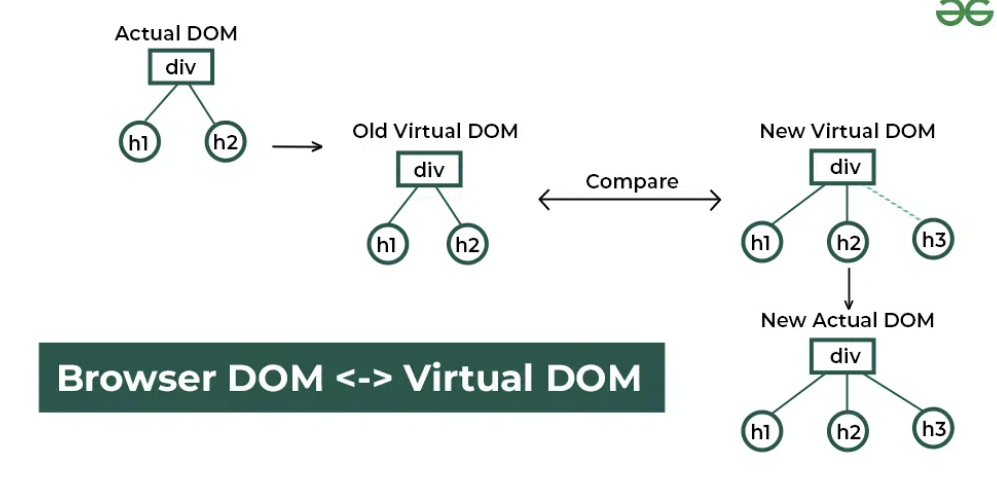
\includegraphics[width=0.7\textwidth]{Images/fundamental/react.png}
    \vspace{12pt}\caption{ReAct Virtual DOM; Source: GeeksforGeeks}\label{fig:react_fe}
\end{figure}
React is a JavaScript library for building user interfaces, created by Meta in 2011 to address the challenges of building large-scale, dynamic web applications. Unlike previous generations of tools that relied on imperative manipulation of the browser's Document Object Model (DOM), React introduced a declarative model utilizing a Virtual DOM. This is a lightweight memory representation of the UI. When the application state changes, React calculates the difference and updates the real DOM efficiently. This approach allows developers to build complex, stateful interfaces that update in real-time without compromising performance, offering some key features:
\begin{itemize}
    \item Component-Oriented Architecture: React encourages breaking the UI into independent, reusable pieces called Components (e.g., a SearchBar, a ContentViewer). This isolation allows for modular development and easier maintenance of the code.
    \item Unidirectional Data Flow: Data flows in a single direction, from parent to child components. This structure makes the application state predictable and easier to debug, which is essential when managing the streaming data from the AI agents.
    \item Rich Ecosystem: Being a library rather than a rigid framework, React allows for the integration of specialized tools for routing, state management, and visualization, providing the flexibility needed to build a custom dashboard.
\end{itemize}

\subsubsection*{AWS}
AWS (Amazon Web Services)~\cite{aws_docs} is a comprehensive cloud computing platform that provides a wide range of services, including computing power, storage, and databases, all needed for the containerized environment to actually run. Further more, for that running containerized applications to be publicly accessible, it needs to be hosted on a cloud platform that expose accessible domain to the internet. AWS provides that, along with various tools and services for managing and orchestrating containerized applications, and since its foundation it has been developing itself to be the infrastructure that brings:

\begin{itemize}
    \item {Scalability:} AWS offers a wide range of services that can be easily scaled up or down based on demand. This allows businesses to handle varying workloads without worrying about infrastructure limitations.
    \item {User-Friendly Interface:} AWS provides a user-friendly web interface and command-line tools that make it easy for developers to manage their resources and deploy applications. This accessibility has contributed to its widespread adoption.
    \item {Flexibility:} AWS supports a wide variety of programming languages, frameworks, and operating systems, allowing developers to choose the tools that best fit their needs. This flexibility has made it a popular choice for a diverse range of applications.
    \item {Global Reach:} With data centers located around the world, AWS allows businesses to deploy applications closer to their users, reducing latency and improving performance. This global infrastructure is a significant advantage for companies with an international user base.
    \item {Security:} AWS provides robust security features, including encryption, identity and access management, and compliance certifications. This focus on security has made it a trusted platform for businesses of all sizes, including those in regulated
    \item {Reliability:} Among the most well\-known cloud providers such as Google, AWS have a strong reputation for reliability, with such few records of failures (esspecially comparing to Google, from my own experience). AWS has a strong track record of uptime and reliability, with multiple availability zones and data centers designed to ensure high availability. This reliability is crucial for businesses that require consistent access to their applications and data.
\end{itemize}
AWS has become a dominant player in the cloud computing market due to its comprehensive service offerings, scalability, user-friendly interface, flexibility, global reach, security features, and reliability. It continues to innovate and expand its services, making it a preferred choice for businesses of all sizes looking to leverage cloud technology for their applications and infrastructure needs. Finally, with a big community and ecosystem, AWS provides extensive documentation, support, and third-party integrations, making it easier for newbies to find resources and solutions for their specific use cases. It is a good start to quickly deploy a reliable scalable system without worrying about the underlying infrastructure, allowing the research to concentrate on the core AI and educational system development.
\subsection{Security: OAuth 2.0 Authorization}

OAuthis a widely used authentication and authorization protocol in backend systems across various programming languages and frameworks. Here are some general benefits of incorporating OAuth into the backend system:

\begin{itemize}
    \item {Security:} OAuth provides a secure way for users to grant third-party applications limited access to their resources without sharing their credentials. This reduces the risk of unauthorized access and protects user data.

    \item {User Experience:} OAuth enables seamless authentication and authorization experiences for users by allowing them to log in to your application using their existing accounts from trusted providers. This eliminates the need for users to create and manage yet another set of credentials.

    \item {Single Sign-On (SSO):} OAuth facilitates single sign-on capabilities, enabling users to access multiple applications and services with a single set of credentials. This improves user convenience and reduces the likelihood of password fatigue.

    \item {Granular Permissions:} OAuth allows you to define and enforce granular permissions for accessing resources. This ensures that third-party applications only have access to the specific resources they need, enhancing security and privacy.

    \item {Scalability:} By offloading user authentication and authorization to OAuth providers, your backend system can better handle scalability challenges. OAuth providers are equipped to handle large volumes of authentication requests efficiently, allowing your application to scale more effectively.

    \item {Standardization:} OAuth is a widely adopted and standardized protocol, supported by major technology companies and libraries across different programming languages. Leveraging OAuth in your backend system ensures compatibility with a broad ecosystem of tools and services.

    \item {Compliance:} OAuth implementations often come with built-in support for compliance with regulatory requirements such as GDPR (General Data Protection Regulation) or HIPAA (Health Insurance Portability and Accountability Act). This can simplify your compliance efforts and reduce legal risks.
    \item {Developer Ecosystem:} OAuth has a large and active developer community, providing extensive documentation, libraries, and support for various 
    programming languages and frameworks, such as PyJWT for protocol schema, e.t.c. This makes it easier for developers to implement OAuth in their backend 
    systems and troubleshoot any issues that may arise.
\end{itemize}

\section{Related Work}

\subsection{Document-Knowledge Modeling}
    Converting documents into structured knowledge representations has become a critical task for so long in the industry and education specifically. To replace manual 
curation in educational contexts, which is time-consuming and not scalable, prior attempts have been focusing on the power of entity extraction, prerequisite relation 
reasoning, and RAG. This has been indeed a fine strategy, given the success of early supervised models like \texttt{PREREQ}~\cite{PREREQ} using latent topic 
representations with Siamese networks to infer course dependencies, which achieved over 70 \% Precision@100 scores on the \texttt{University Course} 
and \texttt{NPTEL MOOC datasets}. However, the traditional methods of entity extraction and relation reasoning often rely on rule-based systems or pure statistical machine learning techniques, 
which can struggle to capture the complexity and nuance of educational content's relationships. Moreover, recent researches~\cite{weller2025theoretical,LostInTheMiddle} have proven that models 
fail drastically to access relevant information when documents exceed a certain length. That is the reason why though prior researches gained impressive results on medium retrieval benchmarks, 
they are not easily applied in industry when it comes to massive and unstructured enterprise data.
\begin{figure}[H]
    \centering
    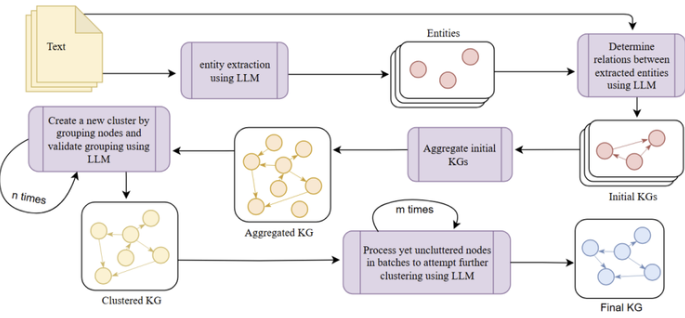
\includegraphics[width=0.8\textwidth]{Images/relate/kggen.png}
    \vspace{12pt}\caption{KGGen with multiturn LLM reasoning, grouping generation}\label{fig:kggen}
\end{figure}
    To address this, LLM-based frameworks have been widely proposed. A prime example is \texttt{KGGen}~\cite{KGGen}, an automated system that utilizes a 
clustering algorithm to group synonymous entities and relations, resulting in denser and better-connected graphs that scored an impressive 81.03\% average 
fact accuracy on the \texttt{MINE-2} (Measure of Information in Nodes and Edges) benchmark. The \texttt{EDC}~\cite{EDC} framework extends this capability by 
extracting, automatically defining schemas, and canonicalizing knowledge triples without predefined schemas, consistently surpassing state-of-the-art baselines on 
complex datasets like \texttt{WebNLG}, \texttt{REBEL}, and \texttt{Wiki-NRE}. 
\begin{figure}[H]
    \centering
    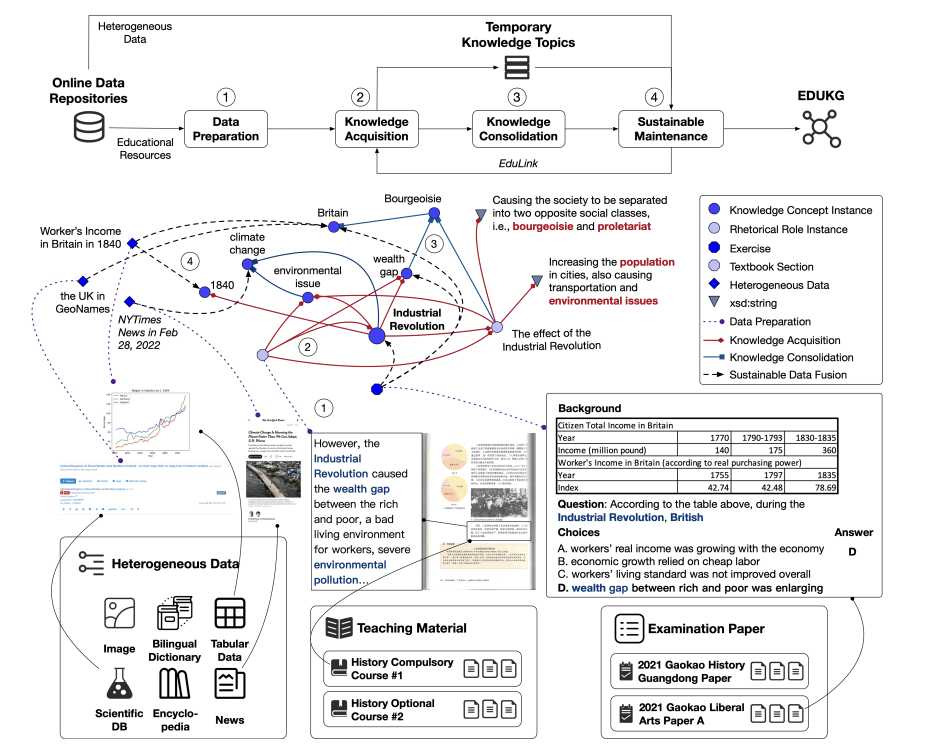
\includegraphics[width=0.8\textwidth]{Images/relate/edukg.png}
    \vspace{12pt}\caption{The end-to-end EduKGPipeline framework for educational knowledge construction and retrieval.}\label{fig:edukgpipeline}
\end{figure}
    However, LLMs have deadly drawbacks. First and most popular of all is the "hallucinations problem" leading to inaccurate, destructurized extractions. To mitigate this, \texttt{GraphJudge}~\cite{GraphJudge} proposes using a fine-tuned open-source LLM as a "judge" to score and filter out incorrect 
knowledge triples generated by naive LLMs. Validated on general (\texttt{REBEL-Sub}, \texttt{GenWiki}) and domain-specific benchmarks (\texttt{SCIERC}, 
\texttt{Re-DocRED}), it achieved over 90\% judgement accuracy. Furthermore, for large-scale educational and enterprise systems requiring cost and latency 
optimization, comprehensive hybrid pipelines have proven highly effective in practices. For instance, \texttt{EduKGPipeline}~\cite{EduKGPipe} establishes 
an end-to-end framework fusing traditional text extraction with transformer-based weighting, demonstrating high precision on educational transcripts from the 
\texttt{CCI dataset}. 
\begin{figure}[H]
    \centering
    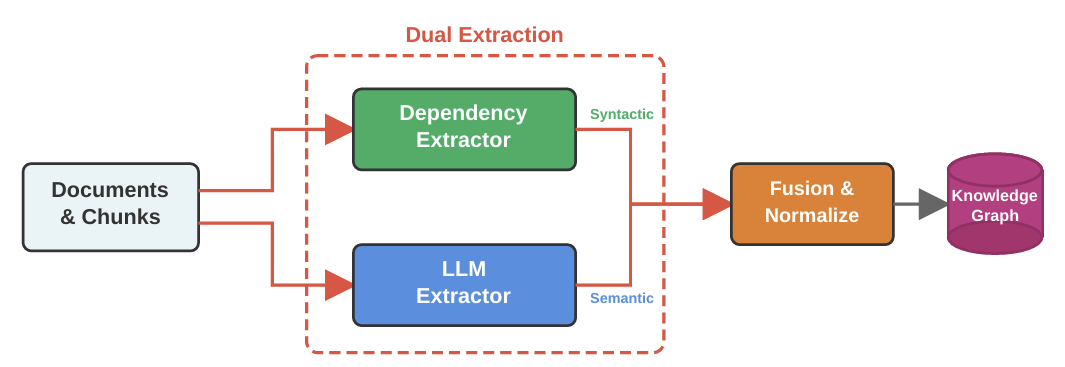
\includegraphics[width=0.8\textwidth]{Images/relate/graphrag hybrid.png}
    \vspace{12pt}\caption{Hybrid architecture of GraphRAG allow minimal cost and guarantee alignment of generated to original context}\label{fig:graph_hybrid}
\end{figure}
Similarly, recent efficient GraphRAG architectures~\cite{GraphRAG} substitute expensive LLM extractions with classical dependency parsing 
to maintain scalability, retaining 94\% of LLM-based performance on \texttt{RAGAS} metrics when evaluated on real-world enterprise datasets like \texttt{CCM} 
(Custom Code Migration). Finally, \texttt{CoDe-KG}~\cite{CoDeKG} utilizes syntactic decomposition to process complex sentences, thereby significantly enhancing 
information recall by an 8-point gain on rare relations across the \texttt{REBEL} and \texttt{WebNLG2} benchmarks.

Another inevitable error lies in the LLMs' limited context length, making it unable to generalize broad knowledge. It is good when discovering short-dependent 
context/entities/relationships in small sections but 
fails for long dependencies of extremely long documents and course information. Trying to inject an excessive amount of information even when cut by windows, 
until now with the current level, only leads to redundant costs from multiple calls, information overload, and decreased accuracy. To uncover hidden relationships 
and deduce learning paths beyond textual information, some studies shifted to an algorithmic approach.
\begin{figure}[H]
    \centering
    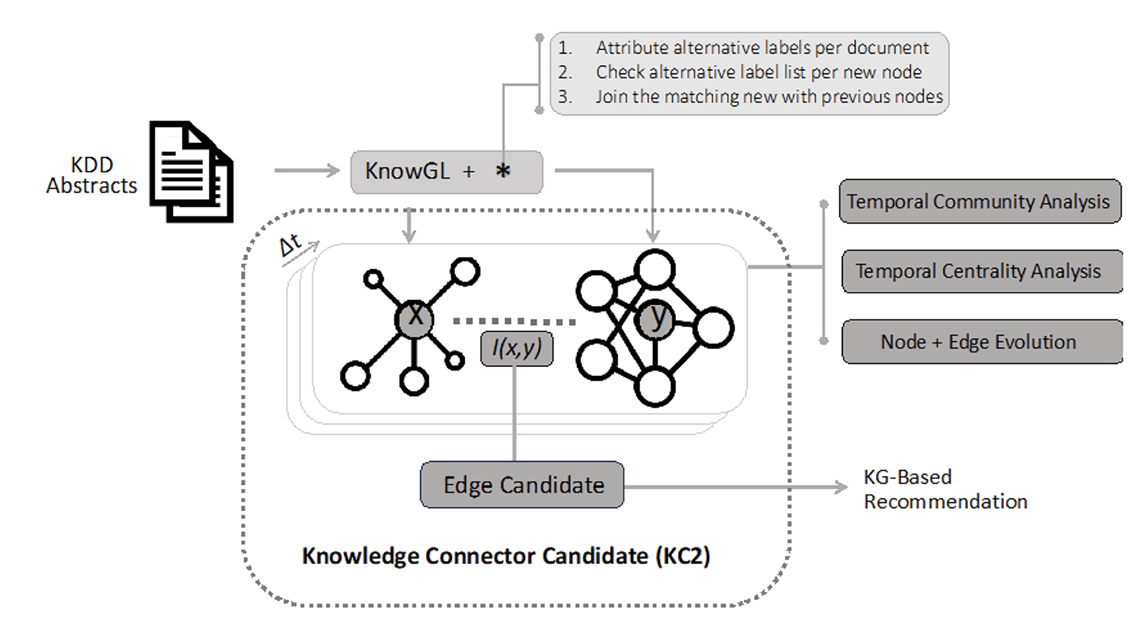
\includegraphics[width=0.8\textwidth]{Images/relate/dkg.png}
    \vspace{12pt}\caption{Dynamic Knowledge Graph (DKG) approach tracking knowledge evolution over time.}\label{fig:dkg}
\end{figure}
The \texttt{Dynamic Knowledge Graph (DKG)}~\cite{DKG} is one of the strongest representative to this approach, analyzing their macroscopic structure becomes crucial. 
It divides KGs into discrete time snapshots and applies network science to track 
knowledge evolution. To recommend optimal learning paths, DKG introduces the \texttt{KC2 (Knowledge Connector Candidate)} algorithm, which uses closeness 
centrality to suggest connections between disconnected knowledge islands. Additionally, to cluster knowledge into logical chapters or modules, the 
\texttt{Leiden}~\cite{Leiden} algorithm is utilized to optimize the CPM quality function, ensuring that knowledge communities are absolutely well-connected 
and not disjointed—a common flaw of the traditional Louvain algorithm.

\subsection{Generative AI in Interactive Teaching}
Bridging the gap between raw document extraction algorithms and end-user educational platforms is the integration of Generative AI and Large Language Models (LLMs). 
The increasing accessibility and reasoning capabilities of Generative AI tools have led to widespread exploration in educational settings, fundamentally 
transforming traditional teaching and learning paradigms~\cite{AI_in_Edu}. Modern LLM agents are proved to be capable of autonomous reasoning, 
tool manipulation, and orchestrating complex academic tasks. 

\subsubsection*{Advances in Educational Agents}
Recent surveys highlight the versatility of LLM agents in automating multifaceted educational workflows, ranging from curriculum design to generating highly contextualized 
feedback~\cite{llm_in_edu}. These agents operate dynamically, leveraging multi-hop reasoning and continuous interaction to adapt to a student's cognitive state. A qualitative study involving educators demonstrated that the core impact of generative models spans three critical pillars: active teaching and learning, administrative automation, and personalized assessments~\cite{AI_in_Edu}. 

A prominent, large-scale empirical example of this shift is the integration of AI within Harvard University's CS50 course. By deploying a suite of specialized 
AI-based software, the course successfully approximated a 1:1 teacher-to-student ratio. Crucially, the system was designed with pedagogical boundaries—guiding 
students toward conceptual understanding rather than merely offering outright code solutions. This constrained autonomy proved highly effective in code explanation, 
style improvement, and administrative querying, demonstrating the practical viability of AI as a ubiquitous teaching assistant~\cite{ai_4_CS50}.

\subsubsection*{Challenges and Deployment Bottlenecks}
Despite the profound opportunities, deploying LLM agents in educational ecosystems introduces substantial systemic and ethical challenges. The inherent probabilistic 
nature of LLMs frequently leads to "hallucinations," where the model confidently generates factually incorrect or pedagogically flawed information. Furthermore, 
there is a significant risk of cognitive offloading, where students develop an overreliance on AI, thereby degrading their independent problem-solving 
skills~\cite{llm_in_edu}. 

From a practitioner's perspective, integrating these models into open-source or institutional infrastructure often encounters severe operational bottlenecks. 
Empirical analyses of LLM-based open-source projects categorize these challenges primarily into model configuration issues, connection instabilities, and feature 
misalignment, all of which hinder seamless deployment~\cite{open_source_isue}. Furthermore, theoretical analyses of LLM representations reveal phenomena such as 
"semantic collapse," where the continuous manifold of the model's activations struggles to maintain stable, logically sound ontologies over continuous, long-term 
reasoning tasks without rigid architectural constraints~\cite{semantic_collapse}. These limitations emphasize the need for robust frameworks to 
tightly navigate the semantic boundaries for AI agents in an academic context.

\subsubsection*{Agentic Workflows}
As educational AI transitions from static next-token prediction to autonomous multi-agent collaboration, ensuring the reliability, alignment, and transparency of 
these systems becomes a critical engineering challenge. Traditional benchmarks, which typically evaluate single-response accuracy, are inadequate for assessing the 
non-linear, multi-step nature of agentic workflows. 

This necessitates the development of rigorous, process-aware evaluation frameworks. Architectures like the Adaptive Evaluation Multi-Agent (AEMA) framework have been 
proposed to address this gap. AEMA provides an auditable, multi-step evaluation mechanism that operates under human oversight, ensuring that the agents' internal 
decision-making processes, tool selections, and collaborative strategies are verifiable and transparent~\cite{AEMA_agentic_eval}. Implementing such verifiable 
frameworks is essential to mitigate the risks of unconstrained autonomy, ensuring that the integration of AI into education remains both trustworthy and pedagogically effective.

\subsection{Educational Intelligent System}
Smart AI based educational systems has leverage from pure research topic and find itself introduced to commercial use. A lot of Intelligent commercial platforms have been 
born recently, and research instituitions have also propose a fully end-to-end pipeline beyond a benchmarked study method. 

In research field,~\cite{EduKG} (along with variants like K12EduKG and MOOC-KG) has been developed to uniformly model knowledge from textbooks and online courses. The~\cite{EduKGPipe} framework automates KG construction from unstructured PDF documents by extracting keywords via Keybert and performing semantic linking with LLMs. 
Furthermore, \texttt{MEduKG} pushes beyond text limitations by integrating multi-modal data into the graph, thereby enhancing the system's comprehensiveness and 
vividness for students.

As mentioned, some systems relating to this field have also reached the market. Popular platforms worldwide like \texttt{Khanmigo} leverage 
Generative LLMs to provide personalized tutoring and real-time feedback, with enormous available resources.
For Vietnamese representative, \texttt{VioEdu} utilizes a manually curated knowledge tree to structure its curriculum, while 
\texttt{EdMicro}, specialized for enterprises, employs a skill matrix to map out learning objectives and prerequisites. 
 These systems represent different approaches to integrating AI into education, each with its own strengths and limitations in terms of scalability, personalization, and content structuring.
Based on practical surveys and evaluation criteria, current educational systems in the market exhibit various characteristics regarding AI and knowledge structuring. A comparative analysis of these platforms is presented in Table \ref{tab:edu_sys}.

\begin{table}[H]
\centering
\resizebox{\textwidth}{!}{
\renewcommand{\arraystretch}{1.4}
\begin{tabular}{|p{8.0 cm}|c|c|c|c|c|}
\hline
\textbf{Criteria} & \textbf{EduKG} & \textbf{Khan Academy} & \textbf{Docebo} & \textbf{VioEdu (FPT)} & \textbf{EdMicro} \\
\hline
\textbf{Adaptive learning:} Personalize the learning process based on needs, abilities, and preferences. & High & High & Low & Medium & Medium \\
\hline
\textbf{Intelligent Recommendations:} Some personalized suggestions courses, videos based on preferences, and areas of improvement. & High & High &  & Low &  \\
\hline
\textbf{Natural language processing for queries:} Based on the questions from learners, it can give out the answer based on the content the LMS has in its DATABASE. & High & Medium & & & \\
\hline
\textbf{Learning analytics/Progress Tracking:} AI-based analytics track and analyze user progress. Can visualize using tracking board, and leaderboard. & Medium & High & High & High & High \\
\hline
\textbf{Text-to-audio content:} Provide audios for text content. & & High & & & \\
\hline
\textbf{Interactive learning method:} Interactive content, such as quizzes, coding exercises, and simulations, can engage learners and reinforce learning. & Low & Low & Medium & Medium & Medium \\
\hline
\textbf{Dynamic KG Reasoning \& Roadmap:} Automatically extract concepts and mathematically reason long-term prerequisite learning paths without manual expert input. & & & & & \\
\hline
\end{tabular}
}
\caption{Comparative analysis of representative educational intelligent systems based on key AI and knowledge features.}\label{tab:edu_sys}
\end{table}

\subsection{Conclusion and Research Gaps}\label{sub:gaps}
During the survey of mentioned representative researches, upon studying from multiple peer reviews and self-reviews of those, this report pinpoints the following core 
research gaps in the current landscape:

\paragraph*{{Limitations in Automation and Cost Optimization:}} All mentioned big systems heavily depend on manually built knowledge trees or skill matrices. Course contents, 
structured and ordered by expertise indexing, but lack inner modelling and semantic makes the system less adaptive to students' needs and preferences, 
leading to good courses recommendations but terrible inner course concept recommendations.
This makes learning path become a linear process and not flexible on the micro scale, with little to no revision and update. 
The lack of automation also limits the scalability of these systems, as manual labeling becomes increasingly impractical as the amount of content grows.
\paragraph*{{Lack of Connectivity and Transparency in Lesson Structures:}} Traditional methods like clustering in text-mining often produce disconnected 
or fragmented knowledge groups. Existing learning platforms typically lack a standard, mathematically proven network algorithm for dividing study modules, leading 
to disjointed learning path that disrupt the learners' cognitive flow.
    
\paragraph*{{Static Roadmap Reasoning and Gap Detection:}} While current LMSs and AI tutors provide generated advice, they are actually still relied on traditional long 
form docs or RAG, lacking the network structure and deterministic approach to map out prerequisites dynamically. The identification of critical "knowledge gaps" remains 
static and reactive, failing to automatically trace back to the fundamental bridge concepts (based on network centrality) that cause student bottlenecks.

So far~\cite{EduKGPipe} and its lineages have made a significant attempt to propose solutions to those mentioned problems with an 
end-to-end pipeline that fuses traditional text extraction with transformer-based weighting.~\cite{DKG} has proposed what~\cite{EduKGPipe} is missing: a mathematical 
efficient community detection method, furthermore solve the connectivity and transparency issues in lesson structures that almost all of previous pipeline encountered. 
However both have their own limitations. The former has no deterministic knowledge mapping, which causes knowledge disruption (even when the graph is not fragmented), 
while the latter pipeline is not as efficient in multistep extraction as the former, thus good for knowledge modeling and analysis but not inference and recommendation. 
Finally, a lot of great proposal here are not widely adapted due to the lack of a comprehensive system that make use of their research project. 

